\documentclass[aspectratio=169,11pt]{beamer}
\usetheme{Madrid}
\usecolortheme{default}
\setbeamertemplate{navigation symbols}{}
\setbeamertemplate{footline}[frame number]
\setbeamercolor{block title}{bg=blue!15,fg=black}
\setbeamercolor{block body}{bg=blue!5,fg=black}

\usepackage[utf8]{inputenc}
\usepackage{amsmath,amssymb}
\usepackage{booktabs}
\usepackage{graphicx}
\usepackage{tikz}
\usetikzlibrary{shapes.geometric,arrows.meta,positioning,fit,backgrounds,decorations.pathreplacing}

\newcommand{\refnote}[1]{{\footnotesize\textcolor{gray}{#1}}}

% ---- fitbox: shrink (never enlarge) a diagram to fit both width and height ----
\newsavebox{\fitboxreg}
\newcommand{\fitbox}[2][0.55]{%
  \sbox{\fitboxreg}{#2}%
  \pgfmathsetmacro{\fitboxWratio}{0.95*\textwidth/\wd\fitboxreg}%
  \pgfmathsetmacro{\fitboxHratio}{#1*\textheight/(\ht\fitboxreg+\dp\fitboxreg)}%
  \pgfmathsetmacro{\fitboxScale}{min(\fitboxWratio,\fitboxHratio,1)}%
  \scalebox{\fitboxScale}{\usebox{\fitboxreg}}%
}

% ---- shared tikz styles (consistent across all diagrams) ----
\tikzset{
  box/.style={rectangle, draw, rounded corners, minimum height=8mm, align=center, font=\small, inner sep=2pt},
  frozen/.style={box, fill=blue!10},
  train/.style={box, fill=orange!20},
  op/.style={box, fill=gray!10},
  data/.style={box, fill=green!10},
  arr/.style={-{Latex[length=2mm]}, thick},
  every picture/.append style={remember picture}
}

\title{EmoMV: Cross-Modal Emotion-Conditioned Music Generation}
\subtitle{Pipeline, Architectures, and Experiments}
\author{EmoMV Project}
\date{\today}

\begin{document}

% =====================================================================
\begin{frame}
\titlepage
\end{frame}

% =====================================================================
\begin{frame}{Motivation}
\begin{itemize}
  \item \textbf{Goal:} given a video clip (or a text prompt) expressing a mood, generate music
  that matches that mood.
  \item \textbf{Constraint:} no fine-tuning budget for any large pretrained model --- not the
  video/text encoders, not the music generator.
  \item \textbf{Constraint:} no instance-level (video, caption) pairs exist --- only shared
  categorical mood labels across independently collected video and text data.
\end{itemize}
\vspace{4mm}
\begin{block}{Approach}
Keep every large pretrained model \textbf{completely frozen}. Train only small adapters that
translate between representations: video/text $\to$ shared mood space $\to$ music-generator
conditioning.
\end{block}
\end{frame}

% =====================================================================
\begin{frame}{Pipeline Overview}
\begin{center}
\fitbox[0.68]{%
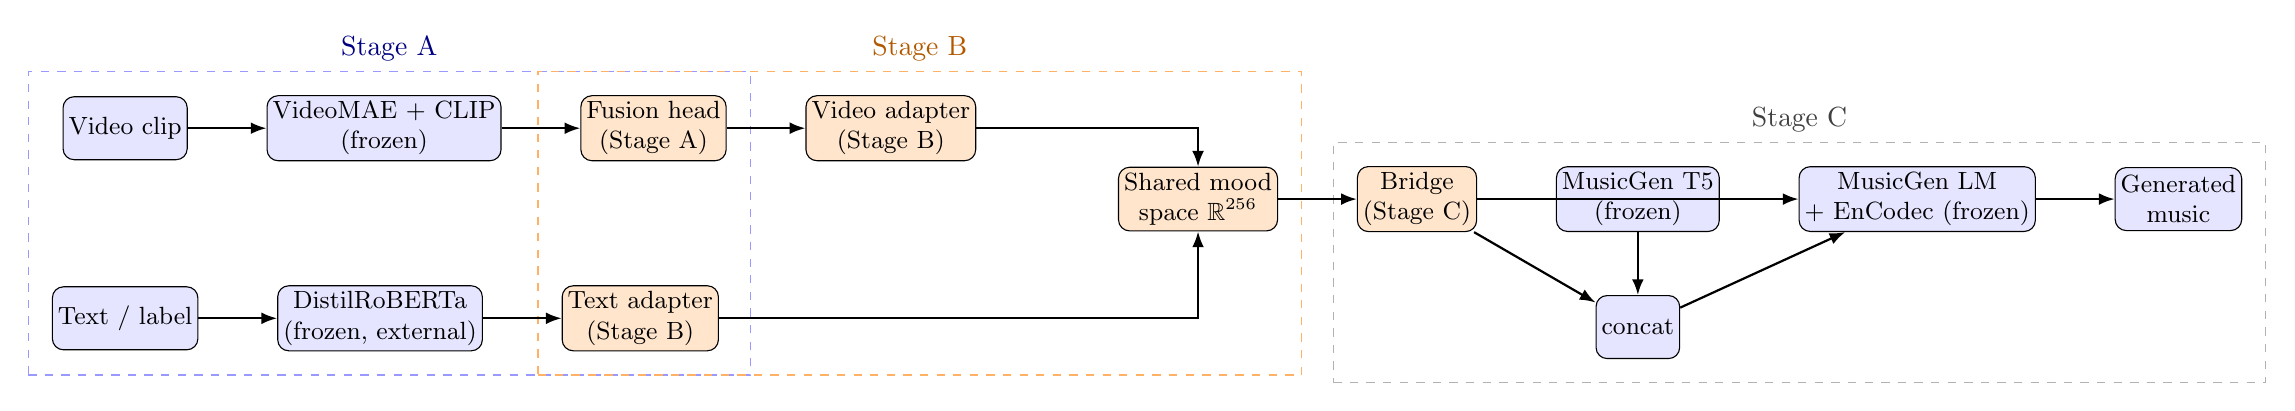
\begin{tikzpicture}[node distance=8mm and 10mm]
\node[frozen] (vid) {Video clip};
\node[frozen, right=of vid] (vmae) {VideoMAE + CLIP\\(frozen)};
\node[train, right=of vmae] (vhead) {Fusion head\\(Stage A)};
\node[train, right=of vhead] (vadapt) {Video adapter\\(Stage B)};

\node[frozen, below=16mm of vid] (txt) {Text / label};
\node[frozen, right=of txt] (roberta) {DistilRoBERTa\\(frozen, external)};
\node[train, right=of roberta] (tadapt) {Text adapter\\(Stage B)};

\node[train, right=18mm of vadapt, yshift=-9mm] (shared) {Shared mood\\space $\mathbb{R}^{256}$};

\node[train, right=of shared] (bridge) {Bridge\\(Stage C)};
\node[frozen, right=of bridge] (t5) {MusicGen T5\\(frozen)};
\node[frozen, below=8mm of t5] (concat) {concat};
\node[frozen, right=of t5] (musicgen) {MusicGen LM\\+ EnCodec (frozen)};
\node[frozen, right=of musicgen] (music) {Generated\\music};

\draw[arr] (vid) -- (vmae); \draw[arr] (vmae) -- (vhead); \draw[arr] (vhead) -- (vadapt);
\draw[arr] (txt) -- (roberta); \draw[arr] (roberta) -- (tadapt);
\draw[arr] (vadapt.east) -| (shared.north); \draw[arr] (tadapt.east) -| (shared.south);
\draw[arr] (shared) -- (bridge); \draw[arr] (bridge) -- (concat); \draw[arr] (t5) -- (concat);
\draw[arr] (concat) -- (musicgen); \draw[arr] (bridge) -- (musicgen);
\draw[arr] (musicgen) -- (music);

\begin{scope}[on background layer]
\node[fit=(vid)(vmae)(vhead)(txt)(roberta), draw=blue!40, dashed, inner sep=3mm, label={[blue!50!black]above:Stage A}] {};
\node[fit=(vadapt)(tadapt)(shared), draw=orange!60, dashed, inner sep=3mm, label={[orange!70!black]above:Stage B}] {};
\node[fit=(bridge)(t5)(concat)(musicgen)(music), draw=gray!60, dashed, inner sep=3mm, label={[gray!50!black]above:Stage C}] {};
\end{scope}
\end{tikzpicture}}
\end{center}
\vspace{2mm}
\centering \textcolor{blue!60!black}{Blue = frozen pretrained model} \quad
\textcolor{orange!70!black}{Orange = trained in this project}
\end{frame}

% =====================================================================
\begin{frame}{Dataset \& Preprocessing}
\begin{columns}
\column{0.5\textwidth}
\textbf{EmoMV dataset} (DS1/DS2/DS3), 5 moods: exciting, fear, tense, sad, relax.
\begin{itemize}
  \item MATCH-only clips kept (video mood = audio mood by construction) --- MISMATCH dropped.
  \item 34 exact duplicates removed (SHA-256), 2 label conflicts resolved.
  \item 20 genuine duration outliers ($>$35s) windowed into 30s chunks.
  \item \textbf{Final manifest: 3{,}189 rows}, 3{,}144 unique videos.
\end{itemize}
\column{0.5\textwidth}
\textbf{Official split leaked} (same source video's segments across train/val/test) --- rebuilt
via grouped, stratified greedy assignment:
\begin{center}
\begin{tabular}{@{}lrrrr@{}}
\toprule
Split & Rows & DS1 & DS2 & DS3 \\
\midrule
train & 2{,}232 & 1{,}870 & 190 & 172 \\
val & 479 & 395 & 59 & 25 \\
test & 478 & 388 & 59 & 31 \\
\bottomrule
\end{tabular}
\end{center}
\end{columns}
\end{frame}

% =====================================================================
\begin{frame}{Building Block: The Transformer Layer}
\begin{center}
\fitbox{%
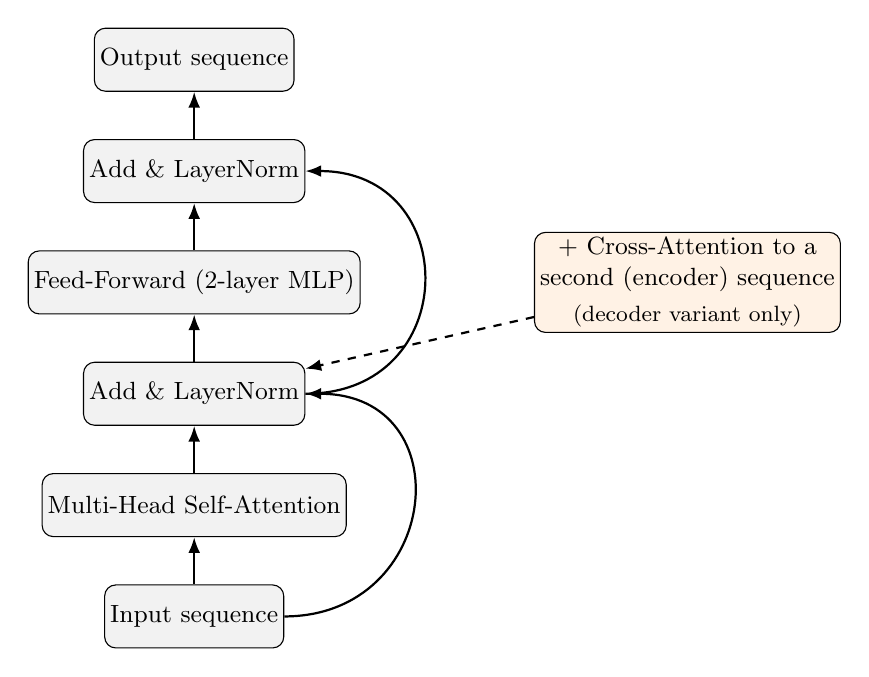
\begin{tikzpicture}[node distance=6mm]
\node[op] (in) {Input sequence};
\node[op, above=of in] (mha) {Multi-Head Self-Attention};
\node[op, above=of mha] (add1) {Add \& LayerNorm};
\node[op, above=of add1] (ffn) {Feed-Forward (2-layer MLP)};
\node[op, above=of ffn] (add2) {Add \& LayerNorm};
\node[op, above=of add2] (out) {Output sequence};
\draw[arr] (in) -- (mha); \draw[arr] (mha) -- (add1); \draw[arr] (add1) -- (ffn);
\draw[arr] (ffn) -- (add2); \draw[arr] (add2) -- (out);
\draw[arr] (in.east) .. controls +(2,0) and +(2,0) .. (add1.east);
\draw[arr] (add1.east) .. controls +(2,0) and +(2,0) .. (add2.east);
\node[op, right=22mm of ffn, fill=orange!10] (cross) {+ Cross-Attention to a\\second (encoder) sequence\\[2pt]\footnotesize (decoder variant only)};
\draw[arr, dashed] (cross) -- (add1);
\end{tikzpicture}
}
\end{center}
\vspace{2mm}
Stacking $N$ of these (encoder: self-attention only; decoder: self- \emph{and}
cross-attention) is the building block behind \emph{every} transformer used or built in this
project --- VideoMAE, CLIP's text tower, RoBERTa, T5, MusicGen's decoder, and our own bridge.
\refnote{Ref: Vaswani et al., ``Attention Is All You Need,'' NeurIPS 2017.}
\end{frame}

% =====================================================================
\begin{frame}{Stage A --- Video Encoder 1: VideoMAE}
\begin{center}
\fitbox{%
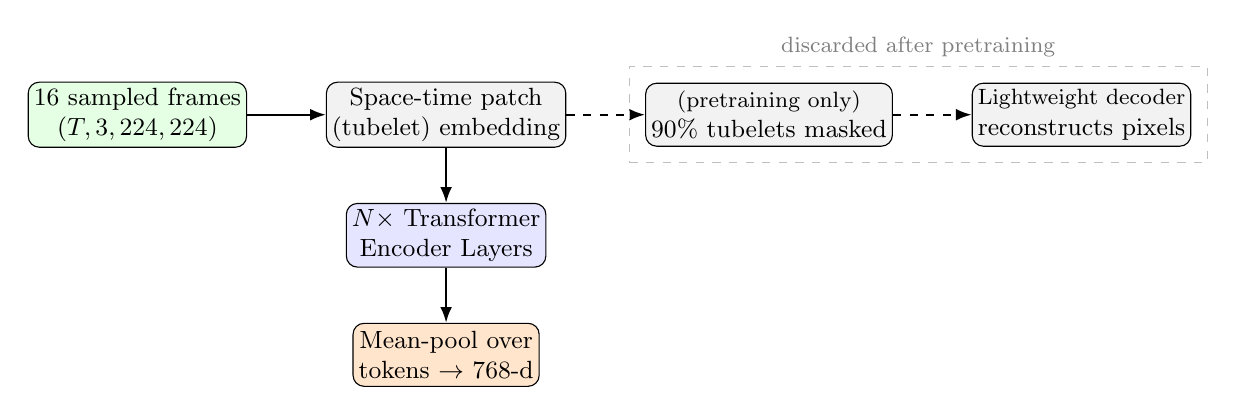
\begin{tikzpicture}[node distance=7mm and 10mm]
\node[data] (vid) {16 sampled frames\\$(T,3,224,224)$};
\node[op, right=of vid] (patch) {Space-time patch\\(tubelet) embedding};
\node[op, right=of patch] (mask) {\footnotesize (pretraining only)\\90\% tubelets masked};
\node[frozen, below=of patch] (enc) {$N\times$ Transformer\\Encoder Layers};
\node[op, right=of mask] (dec) {\footnotesize Lightweight decoder\\reconstructs pixels};
\node[train, below=of enc] (pool) {Mean-pool over\\tokens $\to$ 768-d};

\draw[arr] (vid) -- (patch);
\draw[arr, dashed] (patch) -- (mask);
\draw[arr, dashed] (mask) -- (dec);
\draw[arr] (patch) -- (enc);
\draw[arr] (enc) -- (pool);

\node[fit=(mask)(dec), draw=gray!50, dashed, inner sep=2mm, label={[gray]above:\footnotesize discarded after pretraining}] {};
\end{tikzpicture}
}
\end{center}
\textbf{Our usage:} \texttt{MCG-NJU/videomae-base}, fully frozen, only the encoder is used ---
masking/reconstruction was the \emph{pretraining} objective, not something this project runs.
Output: 768-d embedding per clip.
\refnote{Ref: Tong, Song, Wang, Wang, ``VideoMAE: Masked Autoencoders are Data-Efficient Learners for
Self-Supervised Video Pre-Training,'' NeurIPS 2022.}
\end{frame}

% =====================================================================
\begin{frame}{Stage A --- Video Encoder 2: CLIP}
\begin{center}
\fitbox{%
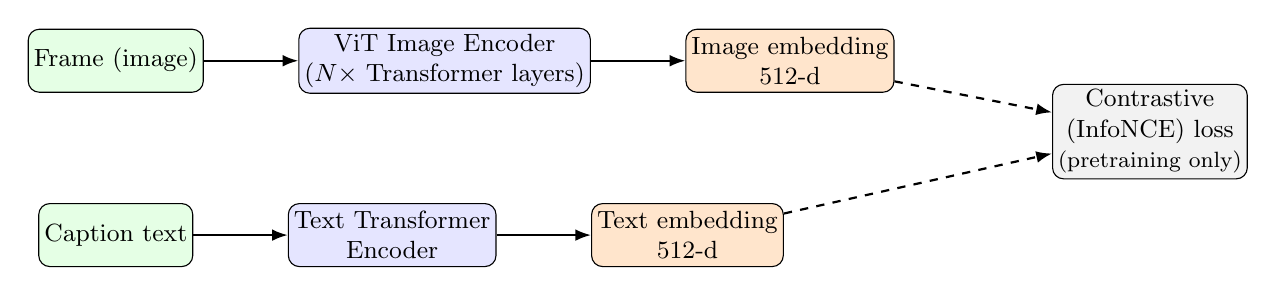
\begin{tikzpicture}[node distance=8mm and 12mm]
\node[data] (img) {Frame (image)};
\node[frozen, right=of img] (vit) {ViT Image Encoder\\($N\times$ Transformer layers)};
\node[train, right=of vit] (iemb) {Image embedding\\512-d};

\node[data, below=14mm of img] (txt) {Caption text};
\node[frozen, right=of txt] (te) {Text Transformer\\Encoder};
\node[train, right=of te] (temb) {Text embedding\\512-d};

\node[op, right=20mm of iemb, yshift=-9mm] (sim) {Contrastive\\(InfoNCE) loss\\\footnotesize (pretraining only)};

\draw[arr] (img) -- (vit); \draw[arr] (vit) -- (iemb);
\draw[arr] (txt) -- (te); \draw[arr] (te) -- (temb);
\draw[arr, dashed] (iemb) -- (sim); \draw[arr, dashed] (temb) -- (sim);
\end{tikzpicture}
}
\end{center}
\textbf{Our usage:} \texttt{openai/clip-vit-base-patch32}, fully frozen. Only the \emph{image
encoder} is used --- per frame, then mean-pooled over 16 frames $\to$ 512-d. The text tower and
contrastive objective are CLIP's own pretraining machinery, not used here.
\refnote{Ref: Radford et al., ``Learning Transferable Visual Models From Natural Language
Supervision,'' ICML 2021.}
\end{frame}

% =====================================================================
\begin{frame}{Stage A --- Baseline Video Encoder: SlowFast}
\begin{center}
\fitbox{%
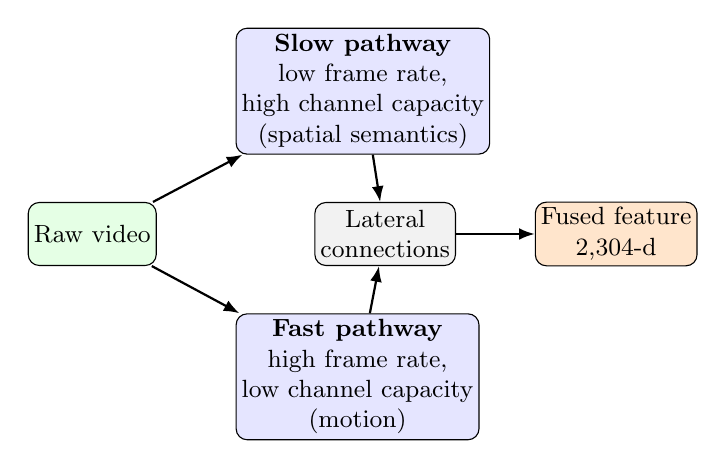
\begin{tikzpicture}[node distance=8mm and 10mm]
\node[data] (vid) {Raw video};
\node[frozen, above right=6mm and 10mm of vid] (slow) {\textbf{Slow pathway}\\low frame rate,\\high channel capacity\\(spatial semantics)};
\node[frozen, below right=6mm and 10mm of vid] (fast) {\textbf{Fast pathway}\\high frame rate,\\low channel capacity\\(motion)};
\node[op, right=20mm of vid, yshift=0mm] (lateral) {Lateral\\connections};
\node[train, right=of lateral] (feat) {Fused feature\\2{,}304-d};

\draw[arr] (vid) -- (slow); \draw[arr] (vid) -- (fast);
\draw[arr] (slow) -- (lateral); \draw[arr] (fast) -- (lateral);
\draw[arr] (lateral) -- (feat);
\end{tikzpicture}
}
\end{center}
\textbf{Our usage:} not re-run --- EmoMV \emph{ships} pre-extracted SlowFast features (2{,}304-d)
per clip; this project only aligns them with its own manifest and trains a small
\texttt{Linear(2304,256)}$\to$ReLU$\to$Dropout$\to$\texttt{Linear(256,5)} MLP on top, as a reference
baseline the VideoMAE+CLIP fusion model must beat.
\refnote{Ref: Feichtenhofer, Fan, Malik, He, ``SlowFast Networks for Video Recognition,'' ICCV 2019.}
\end{frame}

% =====================================================================
\begin{frame}{Stage A --- Text Encoder: (Distil)RoBERTa}
\begin{center}
\fitbox{%
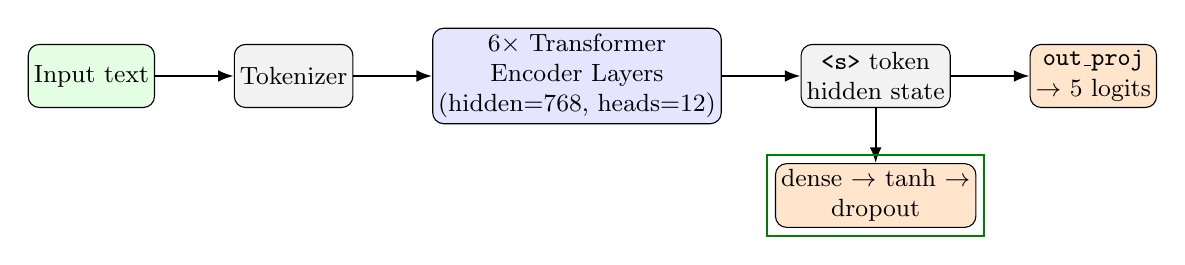
\begin{tikzpicture}[node distance=7mm and 10mm]
\node[data] (txt) {Input text};
\node[op, right=of txt] (tok) {Tokenizer};
\node[frozen, right=of tok] (enc) {6$\times$ Transformer\\Encoder Layers\\(hidden=768, heads=12)};
\node[op, right=of enc] (cls) {\texttt{<s>} token\\hidden state};
\node[train, below=of cls] (head) {dense $\to$ tanh $\to$\\dropout};
\node[train, right=of cls] (out) {\texttt{out\_proj}\\$\to$ 5 logits};

\draw[arr] (txt) -- (tok); \draw[arr] (tok) -- (enc); \draw[arr] (enc) -- (cls);
\draw[arr] (cls) -- (head); \draw[arr] (cls) -- (out);
\node[fit=(head), draw=green!50!black, thick, inner sep=1mm] {};
\end{tikzpicture}
}
\end{center}
\textbf{Our usage:} an already fine-tuned \texttt{distilroberta-base} 5-class mood classifier
(external asset, test macro-F1 $\approx0.80$) is used purely as a frozen encoder. We tap the 768-d
\emph{penultimate} representation (green box: dense+tanh, before \texttt{out\_proj}), verified to
reproduce the model's own logits exactly by manual replay.
\refnote{Ref: Liu et al., ``RoBERTa: A Robustly Optimized BERT Pretraining Approach,'' 2019;
Sanh et al., ``DistilBERT,'' 2019 (distillation methodology).}
\end{frame}

% =====================================================================
\begin{frame}{Stage A --- Fusion Classifier (this project)}
\begin{center}
\fitbox{%
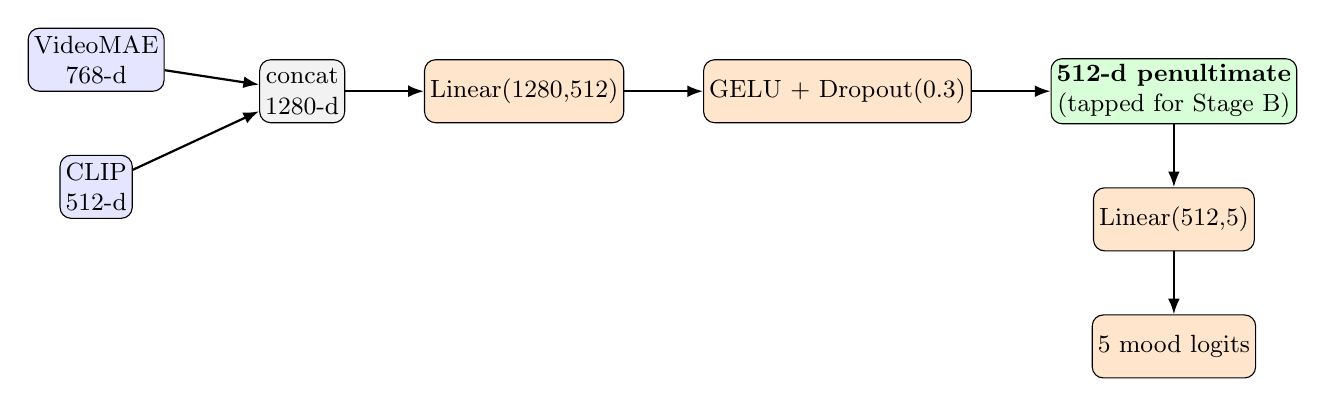
\begin{tikzpicture}[node distance=8mm and 10mm]
\node[frozen] (vmae) {VideoMAE\\768-d};
\node[frozen, below=8mm of vmae] (clip) {CLIP\\512-d};
\node[op, right=12mm of vmae, yshift=-4mm] (concat) {concat\\1280-d};
\node[train, right=of concat] (l1) {Linear(1280,512)};
\node[train, right=of l1] (act) {GELU + Dropout(0.3)};
\node[train, right=of act, fill=green!15] (pen) {\textbf{512-d penultimate}\\(tapped for Stage B)};
\node[train, below=of pen] (l2) {Linear(512,5)};
\node[train, below=of l2] (out) {5 mood logits};

\draw[arr] (vmae) -- (concat); \draw[arr] (clip) -- (concat); \draw[arr] (concat) -- (l1);
\draw[arr] (l1) -- (act); \draw[arr] (act) -- (pen); \draw[arr] (pen) -- (l2); \draw[arr] (l2) -- (out);
\end{tikzpicture}
}
\end{center}
Only this small head is trained; VideoMAE and CLIP remain fully frozen throughout. The green
512-d activation (\emph{after} GELU+Dropout, \emph{before} the final linear layer) is exactly what
Stage B's video adapter later projects from --- not the raw 1280-d concat, not the logits.
\end{frame}

% =====================================================================
\begin{frame}{Stage A --- Results}
\begin{columns}
\column{0.55\textwidth}
\footnotesize
\begin{tabular}{@{}lrrr@{}}
\toprule
Model & Acc & Macro-F1 & W-F1 \\
\midrule
SlowFast & 50.6\% & 0.479 & 0.503 \\
\textbf{Fusion (ours)} & \textbf{80.1\%} & \textbf{0.794} & \textbf{0.803} \\
\bottomrule
\end{tabular}
\vspace{3mm}

\begin{tabular}{@{}lrrr@{}}
\toprule
 & DS1 & DS2 & DS3 \\
\midrule
Fusion acc. & 86.6\% & 52.5\% & 51.6\% \\
\bottomrule
\end{tabular}
\vspace{2mm}

\small A clear domain-shift gap: DS2/DS3 are only 9\% of the data and were flagged as
distributionally different by the EDA's own KS tests.
\column{0.45\textwidth}
\centering
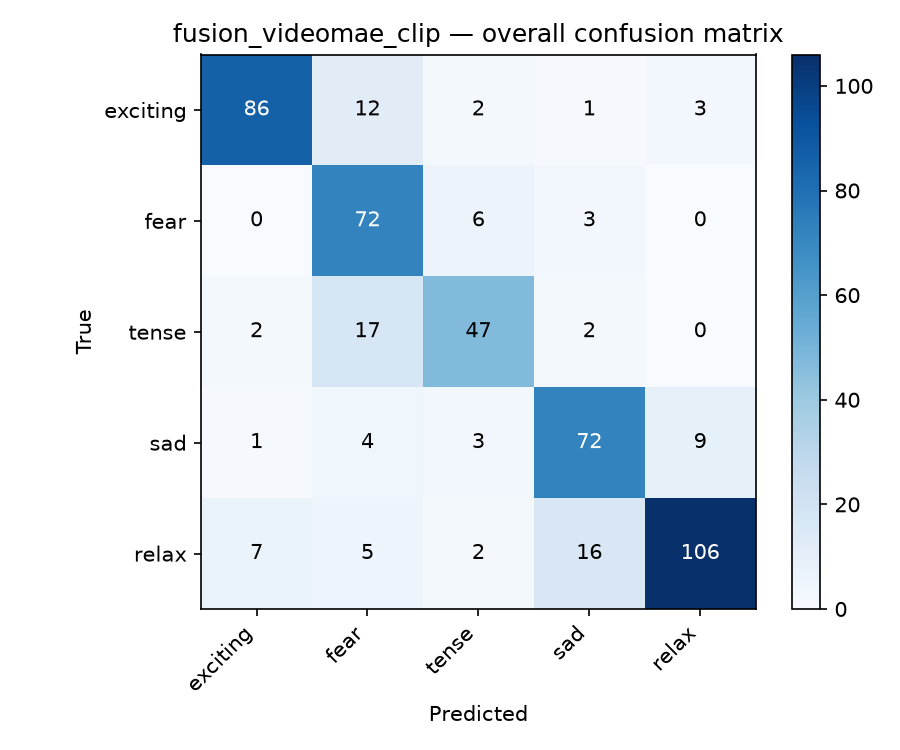
\includegraphics[width=\textwidth]{../evaluation/results/fusion_videomae_clip_confusion_matrix_overall.png}
\end{columns}
\end{frame}

% =====================================================================
\begin{frame}{Stage B --- The Pairing Problem}
\begin{itemize}
  \item Standard CLIP-style contrastive training needs (image, caption) \emph{instance} pairs.
  \item We have none: $\sim$3{,}144 videos and a text corpus, each independently labeled with one
  of the same 5 mood classes --- \textbf{no video$\leftrightarrow$sentence correspondence}.
  \item \textbf{Solution:} use the 5 class-name strings themselves as fixed \emph{text anchors},
  and train with a \textbf{label-anchored supervised-contrastive loss} --- every video is pulled
  toward its class's anchor, every anchor is pulled toward all same-class videos in the batch.
\end{itemize}
\refnote{Generalizes: Khosla et al., ``Supervised Contrastive Learning,'' NeurIPS 2020; temperature
parameterization follows Radford et al. (CLIP), ICML 2021.}
\end{frame}

% =====================================================================
\begin{frame}{Stage B --- Cross-Modal Alignment Architecture}
\begin{center}
\fitbox{%
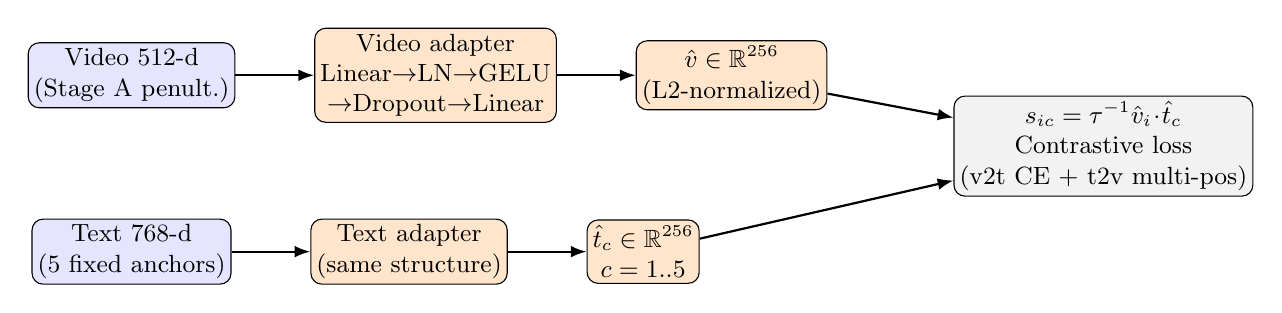
\begin{tikzpicture}[node distance=8mm and 10mm]
\node[frozen] (v) {Video 512-d\\(Stage A penult.)};
\node[train, right=of v] (va) {Video adapter\\Linear$\to$LN$\to$GELU\\$\to$Dropout$\to$Linear};
\node[train, right=of va] (vz) {$\hat v \in \mathbb{R}^{256}$\\(L2-normalized)};

\node[frozen, below=14mm of v] (t) {Text 768-d\\(5 fixed anchors)};
\node[train, right=of t] (ta) {Text adapter\\(same structure)};
\node[train, right=of ta] (tz) {$\hat t_c \in \mathbb{R}^{256}$\\$c=1..5$};

\node[op, right=16mm of vz, yshift=-9mm] (sim) {$s_{ic}=\tau^{-1}\hat v_i\!\cdot\!\hat t_c$\\Contrastive loss\\(v2t CE + t2v multi-pos)};

\draw[arr] (v) -- (va); \draw[arr] (va) -- (vz);
\draw[arr] (t) -- (ta); \draw[arr] (ta) -- (tz);
\draw[arr] (vz) -- (sim); \draw[arr] (tz) -- (sim);
\end{tikzpicture}
}
\end{center}
Only the two small adapters (+ a learnable temperature) are trained; the Stage A encoders behind
them stay frozen. \textbf{Result:} a shared 256-d space where same-mood video/text land close
together.
\end{frame}

% =====================================================================
\begin{frame}{Stage B --- Results}
\begin{columns}
\column{0.45\textwidth}
\begin{center}
\begin{tabular}{@{}lr@{}}
\toprule
Split & V$\to$T Acc. \\
\midrule
Overall & 80.96\% \\
DS1 & 88.66\% \\
DS2 & 50.85\% \\
DS3 & 41.94\% \\
\bottomrule
\end{tabular}
\end{center}
\vspace{2mm}
\small Modality-gap cosine similarity: 0.69--0.73 across classes --- comparable, all positive, no
class catastrophically misaligned.
\column{0.55\textwidth}
\centering
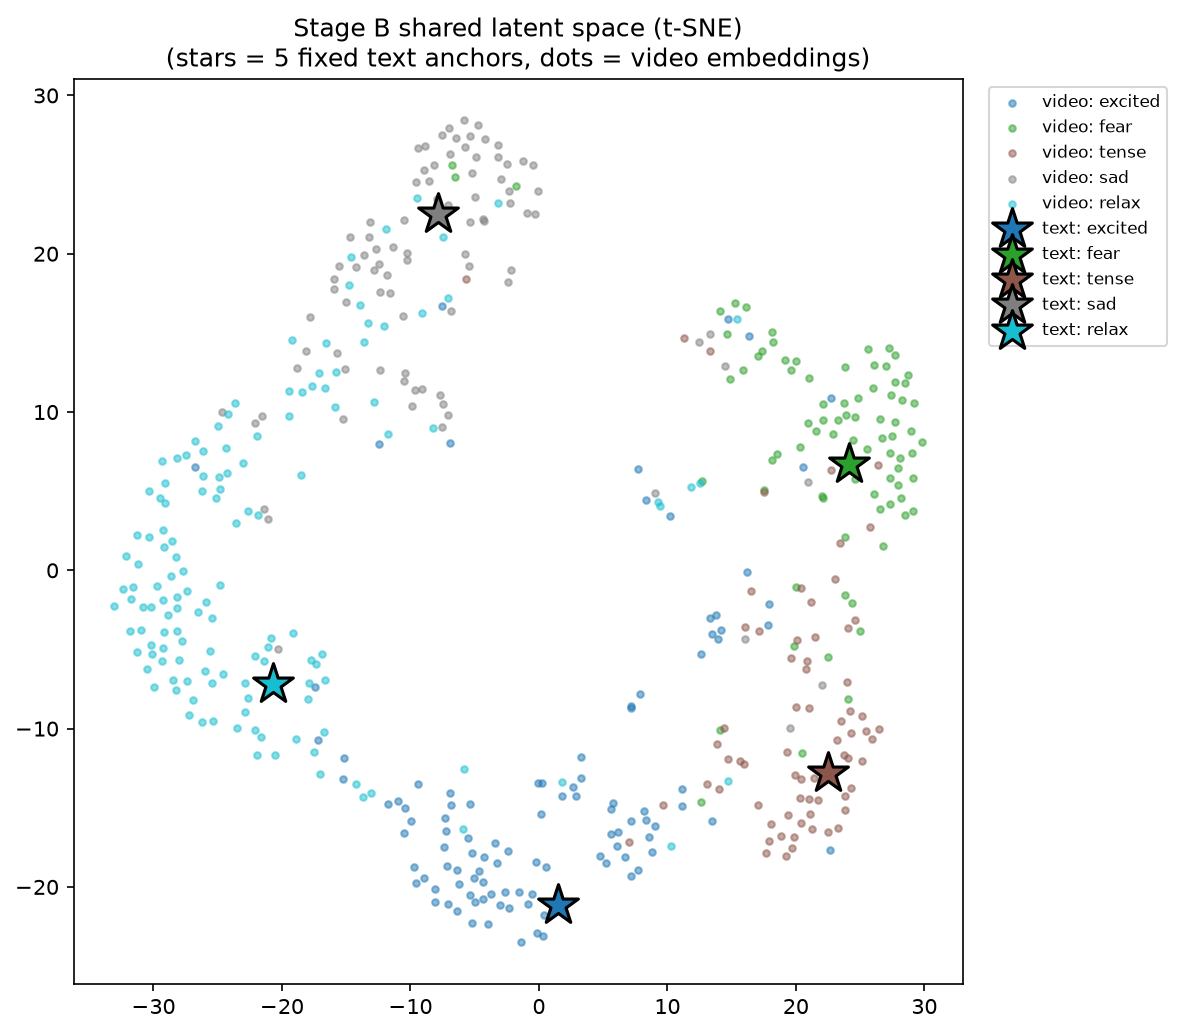
\includegraphics[width=\textwidth]{../evaluation/results/alignment_tsne.png}
\end{columns}
\end{frame}

% =====================================================================
\begin{frame}{Stage C --- The Bridge Network (this project)}
\begin{center}
\fitbox{%
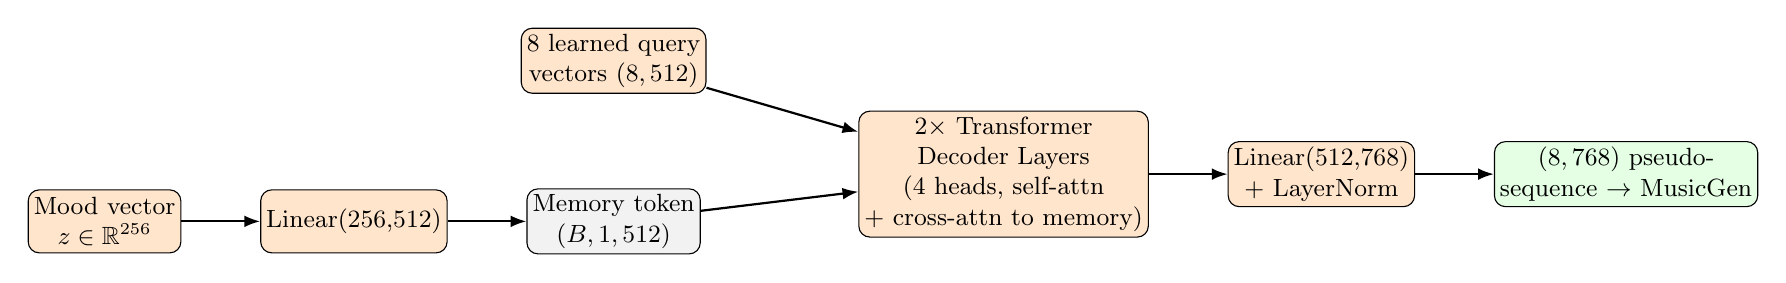
\begin{tikzpicture}[node distance=8mm and 10mm]
\node[train] (z) {Mood vector\\$z\in\mathbb{R}^{256}$};
\node[train, right=of z] (proj) {Linear(256,512)};
\node[op, right=of proj] (mem) {Memory token\\$(B,1,512)$};
\node[train, above=12mm of mem] (q) {8 learned query\\vectors $(8,512)$};
\node[train, right=20mm of mem, yshift=6mm] (dec) {$2\times$ Transformer\\Decoder Layers\\(4 heads, self-attn\\+ cross-attn to memory)};
\node[train, right=of dec] (outp) {Linear(512,768)\\+ LayerNorm};
\node[data, right=of outp] (seq) {$(8,768)$ pseudo-\\sequence $\to$ MusicGen};

\draw[arr] (z) -- (proj); \draw[arr] (proj) -- (mem);
\draw[arr] (q) -- (dec); \draw[arr] (mem) -- (dec);
\draw[arr] (dec) -- (outp); \draw[arr] (outp) -- (seq);
\end{tikzpicture}
}
\end{center}
Built from the generic Transformer-decoder block: 8 learned queries \emph{cross-attend} to a
single memory token derived from $z$, turning one 256-d point into an 8-token sequence shaped
exactly like a T5 conditioning output. Only the bridge is trained; everything it feeds into
(MusicGen) stays frozen.
\refnote{Decoder mechanism: Vaswani et al., NeurIPS 2017.}
\end{frame}

% =====================================================================
\begin{frame}{Stage C --- The Frozen Generator: MusicGen}
\begin{center}
\fitbox[0.4]{%
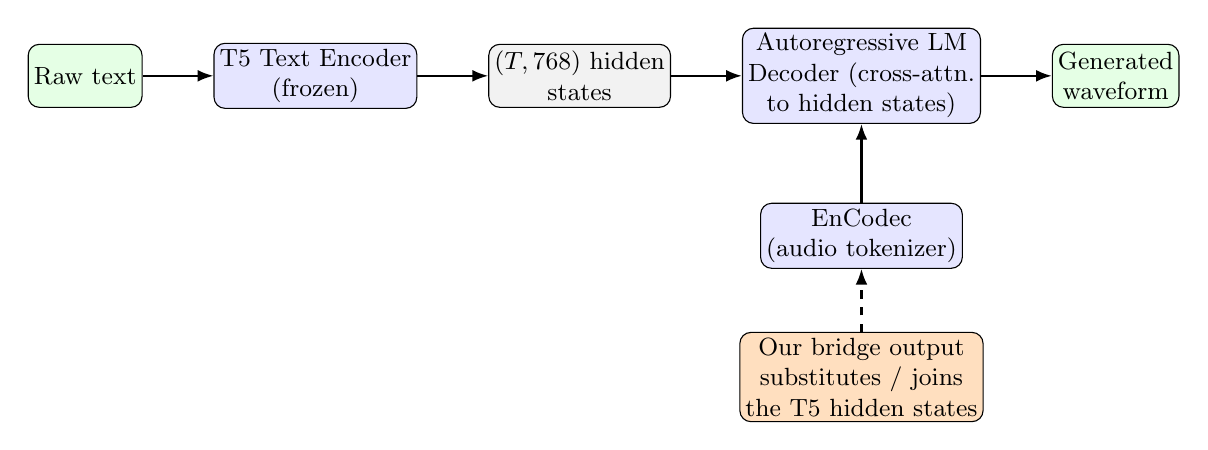
\begin{tikzpicture}[node distance=8mm and 9mm]
\node[data] (text) {Raw text};
\node[frozen, right=of text] (t5) {T5 Text Encoder\\(frozen)};
\node[op, right=of t5] (hid) {$(T,768)$ hidden\\states};
\node[frozen, right=of hid] (lm) {Autoregressive LM\\Decoder (cross-attn.\\to hidden states)};
\node[frozen, below=10mm of lm] (encodec) {EnCodec\\(audio tokenizer)};
\node[data, right=of lm] (wav) {Generated\\waveform};

\draw[arr] (text) -- (t5); \draw[arr] (t5) -- (hid); \draw[arr] (hid) -- (lm);
\draw[arr] (lm) -- (wav);
\draw[arr] (encodec.north) -- (lm.south);
\node[train, below=of encodec, fill=orange!25] (bridge) {Our bridge output\\substitutes / joins\\the T5 hidden states};
\draw[arr, dashed] (bridge) -- (encodec);
\end{tikzpicture}
}
\end{center}
\texttt{facebook/musicgen-small}: an autoregressive transformer over discrete EnCodec audio
tokens. \textbf{Fully frozen} throughout (T5 encoder, EnCodec, LM decoder) --- verified against
the \texttt{transformers} source: supplying \texttt{encoder\_outputs} directly bypasses the
internal T5 call, exactly the hook our bridge uses.
\refnote{Refs: Copet et al., NeurIPS 2023 (MusicGen); Défossez et al., 2022 (EnCodec);
Raffel et al., JMLR 2020 (T5).}
\end{frame}

% =====================================================================
\begin{frame}{Stage C --- Milestone 1 Limitation \& Dual Conditioning}
\textbf{Milestone 1:} bridge output \emph{replaces} T5 conditioning outright ---
\texttt{encoder\_outputs=(bridge(z),)}. Sufficient for \emph{which mood}, but discards genre,
instrumentation, tempo --- anything else in the input text.
\begin{center}
\fitbox{%
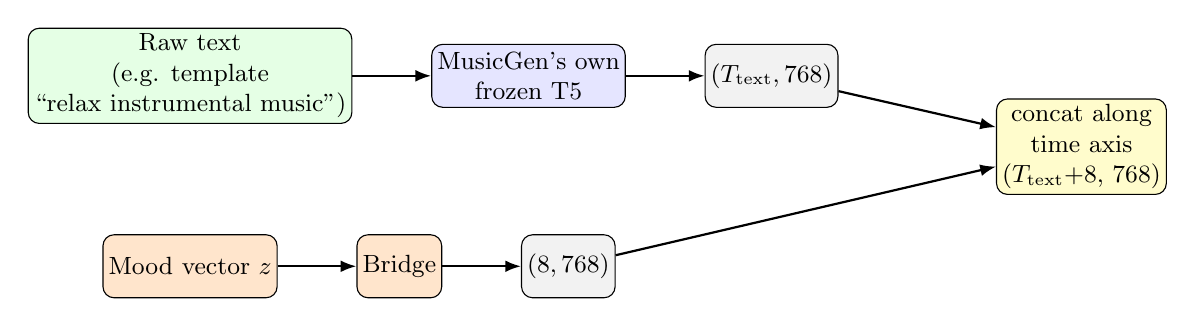
\begin{tikzpicture}[node distance=8mm and 10mm]
\node[data] (text) {Raw text\\(e.g. template\\``relax instrumental music'')};
\node[frozen, right=of text] (t5) {MusicGen's own\\frozen T5};
\node[op, right=of t5] (t5seq) {$(T_{\text{text}},768)$};

\node[train, below=14mm of text] (z) {Mood vector $z$};
\node[train, right=of z] (bridge) {Bridge};
\node[op, right=of bridge] (bseq) {$(8,768)$};

\node[op, right=20mm of t5seq, yshift=-9mm, fill=yellow!20] (cat) {concat along\\time axis\\$(T_{\text{text}}{+}8,\,768)$};

\draw[arr] (text) -- (t5); \draw[arr] (t5) -- (t5seq);
\draw[arr] (z) -- (bridge); \draw[arr] (bridge) -- (bseq);
\draw[arr] (t5seq) -- (cat); \draw[arr] (bseq) -- (cat);
\end{tikzpicture}
}
\end{center}
Only the bridge is retrained under this new objective (\texttt{bridge\_dual\_best.pt}) --- T5
stays frozen (no gradient), and the old single-source checkpoint is kept as a separate ablation
baseline.
\end{frame}

% =====================================================================
\begin{frame}{Stage C --- Three-Way Ablation}
For every test example (text-anchor \emph{and} held-out video), three conditioning variants are
generated and compared by listening:
\begin{center}
\begin{tabular}{@{}lll@{}}
\toprule
Variant & Conditioning & Role \\
\midrule
\textbf{t5only} & $\text{cond}=T5(\text{text})$ & stock MusicGen, zero training \\
\textbf{bridgeonly} & $\text{cond}=\text{bridge}(z)$ & original Milestone-1 design \\
\textbf{combined} & $\text{cond}=[T5(\text{text});\,\text{bridge}(z)]$ & proposed dual conditioning \\
\bottomrule
\end{tabular}
\end{center}
\vspace{3mm}
\begin{itemize}
  \item 40 \texttt{.wav} samples generated across 5 emotions $\times$ \{text, video\} sources.
  \item \textbf{No automatic acoustic metric exists} (no FAD/CLAP) --- evaluation is deliberately
  qualitative: does \emph{combined} keep bridge-only's mood consistency while adding audible
  genre/instrumentation detail from T5?
\end{itemize}
\end{frame}

% =====================================================================
\begin{frame}{Cross-Cutting Finding: Domain Shift}
\begin{center}
\begin{tabular}{@{}lrrr@{}}
\toprule
 & DS1 & DS2 & DS3 \\
\midrule
Stage A (fusion) accuracy & 86.6\% & 52.5\% & 51.6\% \\
Stage B video$\to$text accuracy & 88.7\% & 50.9\% & 41.9\% \\
\bottomrule
\end{tabular}
\end{center}
\vspace{3mm}
\begin{itemize}
  \item DS2+DS3 are only 9\% of the manifest (287/3{,}189 rows).
  \item The EDA's own KS tests found DS1/DS2/DS3 clip-duration distributions significantly
  different --- a genuine domain shift, not a labeling artifact.
  \item The \emph{same} gap reappears independently in two different trained components ---
  strong evidence it reflects the data, not a single model's quirk.
\end{itemize}
\end{frame}

% =====================================================================
\begin{frame}{What Was (and Wasn't) Tried}
\small
\begin{tabular}{@{}p{5.2cm}p{2.6cm}p{4cm}@{}}
\toprule
Experiment & Status & Note \\
\midrule
SlowFast baseline & Done & Superseded by fusion \\
VideoMAE+CLIP fusion & Done & Adopted \\
\texttt{weighted\_sampler} imbalance strategy & Implemented, unused & \texttt{class\_weights} used instead \\
Stage B $D=512$ & Not run & Gated on retrieval plateau (never observed) \\
Auxiliary CE loss (Stage B) & Not implemented & Recommended as collapse safeguard \\
Bridge Milestone 1 (single-source) & Done & \texttt{bridge\_best.pt} \\
Dual conditioning (concat) & Done & \texttt{bridge\_dual\_best.pt} \\
Real per-clip captions & Not available & Template text used instead \\
Cross-attention balance diagnostic & Not implemented & Only manual listening done \\
MusicGen LoRA fine-tuning (Milestone 2) & Not implemented & Needs rented GPU \\
Full MusicGen fine-tuning (Milestone 3) & Not implemented & Needs more paired data \\
\bottomrule
\end{tabular}
\end{frame}

% =====================================================================
\begin{frame}{Limitations \& Future Work}
\begin{itemize}
  \item \textbf{No automatic Stage C metric} --- FAD/CLAP/generated-audio mood classifier would
  replace ``listen manually.''
  \item \textbf{Only 5 fixed text anchors} for Stage B's text side --- no diverse caption corpus,
  so only coarse mood alignment, not fine-grained semantics.
  \item \textbf{Domain shift} (DS1 vs.\ DS2/DS3) unresolved --- more DS2/DS3 data or
  domain-adaptation would help.
  \item \textbf{Compute-gated}: any MusicGen fine-tuning (Milestone 2/3) needs GPU time beyond
  the project's Apple Silicon hardware.
  \item \textbf{Soundtrack audio} used as-is --- may include vocals/dialogue, not pure
  instrumental beds.
\end{itemize}
\end{frame}

% =====================================================================
\begin{frame}{References}
\footnotesize
\begin{itemize}
  \item Vaswani et al. Attention Is All You Need. \emph{NeurIPS}, 2017.
  \item Tong, Song, Wang, Wang. VideoMAE: Masked Autoencoders are Data-Efficient Learners for
  Self-Supervised Video Pre-Training. \emph{NeurIPS}, 2022.
  \item Radford et al. Learning Transferable Visual Models From Natural Language Supervision
  (CLIP). \emph{ICML}, 2021.
  \item Feichtenhofer, Fan, Malik, He. SlowFast Networks for Video Recognition. \emph{ICCV}, 2019.
  \item Liu et al. RoBERTa: A Robustly Optimized BERT Pretraining Approach. \emph{arXiv:1907.11692}, 2019.
  \item Sanh, Debut, Chaumond, Wolf. DistilBERT, a Distilled Version of BERT. \emph{arXiv:1910.01108}, 2019.
  \item Khosla et al. Supervised Contrastive Learning. \emph{NeurIPS}, 2020.
  \item Raffel et al. Exploring the Limits of Transfer Learning with a Unified Text-to-Text
  Transformer (T5). \emph{JMLR}, 2020.
  \item Défossez, Copet, Synnaeve, Adi. High Fidelity Neural Audio Compression (EnCodec).
  \emph{arXiv:2210.13438}, 2022.
  \item Copet, Kreuk, Gat, Remez, Kant, Synnaeve, Adi, Défossez. Simple and Controllable Music
  Generation (MusicGen). \emph{NeurIPS}, 2023.
\end{itemize}
\end{frame}

% =====================================================================
\begin{frame}
\begin{center}
{\Huge Thank you}\\[6mm]
{\large Questions?}
\end{center}
\end{frame}

\end{document}
